\lecture{Process Scheduling I}{2023-03-27}{16:00}{Farzad}{RB LT1}

\section{CPU Scheduling}
CPU Scheduling is a basic requirement of a multiprogrammed operating system. This allows the CPU to be switched between processes, in turn making the computer more efficient. In a system with a single processor, only one process can run at a time; this means the other processes must wait until the CPU becomes free, and is able to be rescheduled, to be able to run. The objective of multiprogramming is to have a process running on the CPU at all times, maximising CPU utilization.

There are different methods of determining how long the process can run on the CPU for before it is removed (this is covered a bit later).

Several processes are kept in memory at one time, some of these will be \verb|READY| to execute, this means they are waiting for time on the CPU and some will be in the \verb|WAIT| state, meaning they require something before they can proceed (generally input or output event). 

CPU scheduling is core to the design \& purpose of the operating system.

\section{Input/ Output Cycle}
The execution of a process alternates between two states: CPU execution (burst) and I/O wait. Process execution begins with a CPU burst and will end with a CPU burst with a system request to terminate execution.

\section{CPU Scheduler}
Whenever a process leaves the CPU and/ or the CPU becomes idle, the operating system has to select one of the processes in the ready queue to be executed. This process is completed by the CPU scheduler. The items (processes) in the ready queue are generally the process control blocks of the processes.
\begin{figure}[H]
    \centering
    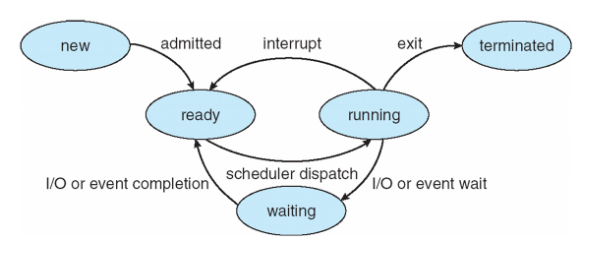
\includegraphics[width=0.7\textwidth]{assets/process-state.png}
    \caption{Process State Diagram}
\end{figure}

\section{Types of Scheduling}
There are two key types of scheduling. There are different algorithms which implement these different types of scheduling (these will be covered later on).
\subsection{Non-Preemptive Scheduling}
In non-preemptive scheduling, a process cannot be stopped mid execution, unless it needs something (eg input from user), in which case it will be stopped and placed on the ready queue. This means that unless the process switches to the \verb|WAIT| state or it terminates, then there is no way to stop it. No choices are made in terms of which process to execute next, one is picked from the ready queue. This scheduling method was used by Windows version 3.x.

\subsection{Preemptive Scheduling}
In preemptive scheduling, if a process with higher priority than that executing arrives into the ready queue then the currently executing process will be stopped and the higher priority one will be given the CPU to execute on. Preemptive scheduling decisions will take place when either a process switches from the running state to the waiting state; or when a process switches from the wait state to teh ready state. There are choices in terms of scheduling. There may also be a requirement for specialist hardware - for example a timer. Windows 95 and all subsequent versions of Windows have used this type of scheduling. 

\section{Scheduler}
A \textit{scheduler} is a piece of systems software which handles process scheduling in a number of ways. Their role is to look at processes submitted to the system and decide which processes to run. 
\begin{description}
    \item[Long Term Scheduler] looks at the big picture. This works out the bits of the programmes which run in what sequence and how many processes stay in the ready queue. This happens away from the CPU. 
    \item[Medium Term Scheduler] processes movement between the wait queue and ready queue.
    \item[Short Term Scheduler] decides which process from the ready queue is the next for execution and the order of execution for the other processes in the ready queue. 
\end{description}

\section{Dispatcher}
The dispatcher is a program which gives the process control over the CPU after it has been selected by the short term scheduler. This involves three things

\begin{enumerate}
    \item Switching Context
    \item Switching to User Mode
    \item Jumping to the proper location in the user program to restart that program
\end{enumerate}

\section{Scheduling Criteria}
\begin{description}
    \item[CPU Utilization] we want to keep the CPU as busy as possible
    \item[Throughput] this is the number of processes that complete their execution per time unit
    \item[Turnaround Time] this is the amount of time it takes to execute a particular process
    \[\text{Turnaround Time} = \text{Exit Time} - \text{Arrival Time}\]
    \item[Waiting Time] this is the amount of time a process has been waiting in the ready queue. 
    \[\text{Waiting Time} = \text{Turnaround Time} - \text{Burst Time}\]
    \item[Response Time] is the amount of time it takes from when a request was submitted until the first response is produced
\end{description}

\section{Scheduling Algorithms}
We will explore six scheduling algorithms over the remainder of this lecture and the next lecture.
\subsection{First Come, First Served (FCFS)}
This scheduling algorithm works by allocating the CPU to the process which arrives first. Processes are stored in a Queue which operates as First In First Out (FIFO). When a new process enters the ready queue, its process control block is linked to the tail of the queue. When the CPU is free, it is allocated to the process at the head of the queue. The newly running process is then removed from the queue.

Once the CPU has been allocated to a process, the process keeps control of the CPU until it releases the CPU either by terminating or requesting I/O (which would result in it being put in the \verb|WAIT| queue).

\begin{link}{FCFS Order Of Execution}
See Week 19 slides on Moodle for an example process execution order with different length processes in different orders.
\end{link}

\subsection{Shortest-Job-First Scheduling (SJF)}
This scheduling algorithm works by executing the CPU to the process with the shortest execution time first. It gives the minimum average waiting time for a given set of processes; however it needs to know the length of all the processes in the ready queue. 

SJF can also be preemptive and works as preemptive is described above. 